%\documentclass{llncs}
\documentclass[10pt]{article}
\usepackage{amssymb}
\usepackage{amsmath}
\usepackage{amsfonts}
\usepackage{algorithm}
\usepackage{algpseudocode}
\usepackage{url}
\usepackage{paralist}
\usepackage{multirow}
\usepackage{graphicx}
\usepackage[draft,margin]{fixme}

\oddsidemargin=0in                % Left margin minus 1 inch.
\evensidemargin=0in                % Same for even-numbered pages.
\textwidth=6.3in                % Text width (8.5in - margins).
\topmargin=0in                    % Top margin minus 1 inch.
\headsep=0.2in                    % Distance from header to body.
\textheight=8in                    % Body height (incl. footnotes)


%\usepackage{float}

%\newtheorem{dfn}{Definition}{}
%\newtheorem{thm}[dfn]{Theorem}{}
%\newtheorem{cor}[dfn]{Corollary}{}
%\newtheorem{prb}{Problem}{}
%\newtheorem{lem}[dfn]{Lemma}{}
%\newtheorem{algx}[dfn]{Algorithm}{}

\newcommand{\bigo}{\mathcal{O}}
\renewcommand{\mod}{\text{ mod }}
\newcommand{\E}{\mbox{\rm \bf{E}}}
\renewcommand{\Pr}{\mbox{\rm \bf{Pr}}}
\newcommand{\Var}{\mbox{\rm \bf{Var}}}
\newcommand{\Xac}{X_{(a,c)}}
\newcommand{\mcA}{\mathcal{A}}
\newcommand{\mcB}{\mathcal{B}}
\newcommand{\mcC}{\mathcal{C}}

\newcommand{\ordo}[1]{{\cal O}\left(#1\right)}
\newcommand{\ordop}[1]{{\cal O}^*\left(#1\right)}
\newcommand{\calG}{\mathcal{G}}
\newcommand{\calH}{\mathcal{H}}
\newcommand{\calE}{\mathcal{E}}
\newcommand{\calX}{\mathcal{X}}
\newcommand{\calS}{\mathcal{S}}
\newcommand{\calT}{\mathcal{T}}
%\newcommand{\qed}{\hfill \ensuremath{\Box}}



\newtheorem{proof}{Proof}
\newtheorem{defx}{Definition}
\newtheorem{lemmx}{Lemma}
\newtheorem{thmx}{Theorem}
\newtheorem{algx}{Algorithm{\\}}
\newtheorem{procx}{Procedure}

\newenvironment{procedure}{\begin{procx}\em \footnotesize}{\end{procx}}

% These are used indirectly by the following group of new environments


%%\newcommand{\e}{\epsilon}
\begin{document}


\title{Does past stock performance matter in investing?}
\date{}
\author{Konstantin Kutzkow and Kevin Tierney}
\maketitle
\begin{abstract}
In our project we investigate the impact of past stock data on future price
movement. We consider two different approaches for predicting the future stock
behavior: supervised learning based on feature vectors built
from technical analysis indicators and sequence mining for discovering
frequent patterns of stock price movements for a given stock. 
\end{abstract}
\section{Introduction}

Stock market investors rely heavily on stock \emph{technicals} to guide their
investing, which are a wide range of formulas that seek to offer advice on a
stock based on the stock's past performance. Technicals differ from stock
\emph{fundamentals} in that fundamentals are statistics about a company itself,
its quarterly earnings, its debt ratio, etc, whereas technicals are derived
solely from the trading of a company's stock.

Given the ubiquity of the use of technicals in investing, one might think that
their predictive value is a given. The literature indicates that certain
technicals do have a predictive value~\cite{brock1992}, but it is still not
clear under what circumstances their predictive value holds, or whether certain
combinations of technicals offer better prediction of stock price.

To this end, we have developed two data mining approaches to investigate the
usefulness of technicals for an average investor, i.e. an investor that uses a
middle to long term trading strategy over the period of weeks and months. We
first use supervised learning to learn a classifier that can predict when a
stock should be bought or sold based on stock technicals leading up to a day of
trading. We then use frequent pattern mining to try to learn rules for trading
that an average investor could use on a day to day basis.
% 
% This paper is organized as follows. First we present the data sources and
% features we used in Section~\ref{sec:data}, followed by an overview of our
% supervised learning approach and its results in
% Section~\ref{sec:supervisedlearning}. We continue with our frequent pattern
% mining approach and its results in Section~\ref{sec:freqpattern} and conclude
% in Section~\ref{sec:conclusion}.


\section{Data}
\label{sec:data}
We gathered publicly available data from Yahoo! Finance\cite{Yahoo} for
different stocks in two sectors, basic materials and technology. The basic
materials sector consists of companies involved with the discovery, development
and processing of raw materials into consumer and industrial goods, such as
food and chemical production. The technology sector contains stock data for
companies in areas like software development, electronics manufacturing, and
other businesses related to information technology. We screened the stocks in
this sector based on two criteria, 
\begin{inparaenum}[\itshape i\upshape)]
    \item stocks must be a member of the S\&P 500, a list of the top 500 companies in the NYSE and NASDAQ exchanges, and
    \item stocks must have been listed in the stock market since January, 2005.
\end{inparaenum}
We chose these criteria to match the investment strategies of average
investors who prefer well-known, large companies that have been around for a
number of years. Our data set consists of 42 stocks from the technology sector
and 31 stocks from basic materials.

We chose these two sectors because they contain two different classes of
companies: \emph{non-cyclicals} and \emph{cyclicals}. No single sector of
stocks contains only one class of companies, however a number of companies in
the basic materials sector are non-cyclicals, i.e. their stock price does not
correlate strongly with the strength of the economy. Companies such as Kraft
Foods (KFT), a maker of cereals and other consumer goods, and Altria Group
(MO), a maker of cigarettes, tend to profit regardless of the state of the
economy, as people continue to eat and smoke even during recessions.

Technology stocks, on the other hand, are often heavily dependent on the amount
of disposable income consumers have, which varies with the economy. In
recessionary periods, consumers do not buy as many electronics, and the price
of technology stocks sag. The technology sector includes companies like
Microsoft (MSFT), Apple (AAPL) and Dell (DELL), which are heavily involved in
retail electronics.

\subsection{Data preprocessing}
In our case data preprocessing is a straightforward task since for each stock
we are provided with a csv file consisting of the following data for each
stock on each trading day: opening price, closing price, highest and lowest
price and the volume, which measures how many times a stock as bought and sold,
for the day. We directly use the numerical values in order to compute technical
analysis indicators and to label days, respectively longer time periods, in a
way describing in an informative manner the behavior of the stock for the
considered time interval. Note that since our data contains no missing or
inconsistent values no data cleaning is necessary.

\subsection{Features}

We used a number of well-known technicals indicators as features. For the
description of the features, we use the following notation for stock data. Let
$c_i, l_i, h_i,$ and $v_i$ be the closing price, daily low, daily high and
volume of day $i$, respectively. Most of these features are calculated over a
period $n$ that starts on a day $s$.
\vspace{-0.35cm}

\paragraph{Simple Moving Average (SMA)} Let $SMA(n, s) =
\frac{1}{n}\sum_{i=s}^{s + n} c_i$, where $n$ is the period of the SMA and $s$
is the start day of the period. We use a period of 200 days, which is a
standard period for the SMA. In addition, we compute the change in the SMA over
the past 20 days with $\frac{SMA(200, i)}{SMA(200, i - 20)}$ in order to determine
whether the stock has been increasing or decreasing in value.
\vspace{-0.35cm}

\paragraph{Exponential Moving Average (EMA)} Let $EMA(n, s) = \alpha c_i + (1 -
\alpha)(EMA(n - 1, s + 1))$, where $\alpha = \frac{2}{n +
1}$. We use a standard period of 50 days along with the direction of
the EMA using $\frac{EMA(50, i)}{EMA(50, i - 20)}$.
\vspace{-0.35cm}

\paragraph{Relative Strength Index (RSI)} Let $RSI(n, s) = \frac{EMA(U(n,
s), 14)}{EMA(D(n, s), 14)}$, where $U = \{c_i - c_{i-1} | (c_i - c_{i - 1}) >
0, s < i \leq s + n\}$ and $D = \{|c_i - c_{i-1}|$ $|$ $(c_i - c_{i - 1}) < 0,
\forall s < i \leq s + n\}.$ Note that in a slight abuse of notation, we
indicate that the EMA is to be taken over the sets $U$ and $D$ with a period of
14 days. The sets $U$ and $D$ represent periods of increasing stock price and
decreasing stock price respectively.
\vspace{-0.35cm}

\paragraph{Williams Percent R (W\%R)} Let $W\%R(n, s) = \frac{h^* - c_s}{h^* -
l^*}$, where $l^* = argmax_{l_i}\{l_i, s \leq i \leq s + n\}$ and $h^* =
argmax_{h_i}\{h_i, s \leq i \leq s + n\}$. The values $h^*$ and $l^*$ represent
the highest high and the lowest low during the period. We use a period of 60
and 10 days for our features.
\vspace{-0.35cm}

\paragraph{Stochastic Oscillator (SOSC)} Let $SOSC(n, s) = \frac{c_s - l^*}{h^*
- l^*}$, where $h^*$ and $l^*$ are defined as in Williams Percent R. The
stochastic oscillator is very similar to Williams Percent R, but provides a
slightly different view of the same data. We use a stochastic oscillator with
period 20 days, along with $\frac{SOSC(20, i)}{SOSC(20, i - 20)}$ to determine
the movement of the SOSC over time.
\vspace{-0.35cm}

\paragraph{Commodity Channel Index (CCI)} Let $CCI(n, s) = \frac{t_i -
SMA(t_i, n, s)}{\sigma(t_i)}$, where $t_i = \frac{h_i + l_i + c_i}{3}$ is the
``typical price''. The CCI is normally multiplied by $\frac{1}{0.015}$, but since it is constant, we have removed it.
\vspace{-0.35cm}

\paragraph{Volume Moving Average (VMA)} Let $VMA(n, s) =
\frac{1}{n}\sum_{i=s}^{s + n} v_i$, which is a measure of the average volume of
a stock. We use a standard period of 200 days, and include a feature
$\frac{VMA(200, i)}{VMA(200, i - 20)}$ that measures the change of the VMA over
the past 20 days.

\section{Supervised learning}
\label{sec:supervisedlearning}

We perform supervised learning by splitting the data from a stock into a three
year training set beginning on January 3, 2005 and ending on January 2, 2008,
and a two year testing set beginning on January 2, 2009 and ending on January 3,
2011. We separate the training set from the testing set to ensure that none of the
features computed for the testing set overlap any days in the training set and,
thus, taint the testing set with information that was used to build our
classifier.

Our training set is labeled with five different labels: Strong Buy, Buy, Hold,
Sell, Strong Sell. We use these five labels in order to allow a trader using
this machine learning code to exercise discretion over when to perform a trade.
The labels provide guidance outside of just the confidence of the classifier.
In order to label days, we calculate the average profit or loss of buying a
stock on a particular day and selling it any of the following 30 days of
trading. We then take the average profit or loss calculated for each day, and
label each day according to where it falls in the distribution of profits and
losses. We label the bottom 5\% of days with the label ``Strong Sell'', the
next 20\% of days with ``Sell'', the next 50\% with ``Hold'', the following
20\% with ``Buy'' and the top 5\% with ``Strong Buy''. Note that due to the
volatility of stocks, there are always some periods that are more desirable
than others, even with a stock that is constantly moving upwards. We use this
labeling strategy because it attempts to find days for buying a stock that are
relatively robust. That is, the days following a buy or strong buy label are
likely to provide a profit, and days following a sell label are likely to
result in a loss.

We compared several different supervised learning algorithms to see which could
provide the largest monetary gain on our dataset. The algorithms we show are
Naive Bayes, a Multilayer Perceptron and a Support Vector Machine
(SVM) with a polynomial kernel. using the WEKA library~\cite{Weka}. We used
default parameters and performed no tuning, as the WEKA algorithms are well
tuned for a wide range of applications.

The Naive Bayes algorithm trains a simple classifier based on Baye's theorem,
which predicts the probability of the value of a random value given some
independent evidence\footnote{In spite of the independence assumption, Naive
Bayes can be used on problems where the features contain dependencies.}. A
class label is assigned to a feature vector by computing the maximum
likelihood estimations of the probabilities for each class.

Multilayer Perceptrons work by creating a network of perceptrons in which an
input layer accepts a feature vector, a hidden layer processes data from the
input layer, and then passes data on to an output layer which predicts a class
label. The Multilayer Perceptron in WEKA uses backpropagation to attempt to
adjust each perceptron's weight to maximize the likelihood of a correct label
prediction by the network.

SVMs~\cite{vapnik2006estimation} are a classification method that maps features from
their original space into a higher dimensional space in which a separation
hyperplane can be found between two class labels. SVMs utilize the \emph{kernel
trick} to perform the mapping.

% Measuring gain

\subsection{Results} 
\label{sec:slresults}

\begin{table}
    \begin{center}
    \begin{tabular}{|c|c|c|c|c||c|c|c|c|}
        \hline
        \multirow{2}{*}{} & \multicolumn{4}{c||}{Technology} & \multicolumn{4}{c|}{Basic Materials} \\
        \cline{2-9}
                        & Avg. & Stdev & Min & Max & Avg. & Stdev & Min & Max\\
        \hline
        Naive Bayes & 14.3 & 6.4 & 6.7 & 36.3 & 11.8 & 3.3 & 4.6 & 24.1 \\
        \hline
        Multi. Perceptron & 14.2 & 5.3 & 9.0 & 33.6 & 11.0 & 2.3 & 4.7 & 16.4 \\
        \hline
        SVM & 11.3 & 5.0 & 6.5 & 34.3 & 10.8 & 2.4 & 9.8 & 22.5 \\
        \hline
        Buy \& Hold & 21.9 & 10.7 & 7.3 & 58.8 & 13.3 & 4.0 & 4.6 & 24.6 \\
        \hline
    \end{tabular}
    \end{center}
    \vspace{-0.5cm}
    \caption{A comparison of different machine learning algorithms to a Buy \&
    Hold strategy. All values are in thousands, with the Avg. column showing
    the average amount of money at the end of the testing period after starting
    with \$10,000 and using a disciplined trading strategy. The min and max
    columns show the minimum and maximum amount of money left over all stocks
    in the sector.}

    \label{tab:testresults}
    \vspace{-0.1cm}
\end{table}

We evaluated the performance of each classifier with a simulation of stock
trading based on the output of the classifier. We start the testing period with
\$10,000 and receive a label for each day from the classifier. If the label is ``Strong Buy'',
we purchase as many shares as we have money for. Conversely, if the label is
``Strong Sell'' we sell all the shares currently owned. If the label is ``Buy''
we attempt to buy \$2,500 worth of shares. If the label is ``Sell'', we attempt
to sell \$2,500 worth of shares.

Table~\ref{tab:testresults} show the results of our experiments. The buy \&
hold strategy involves purchasing a stock at the beginning of the testing
period and not selling it until the end. Buy \& Hold outperforms all of our
classifiers, earning on average \$21,900 from \$10,000 in the technology sector
and \$13,300 in the basic materials sector. The simple buy \& hold strategy is
able to outperform even our best classifier \$7,600 in the technology sector
and by \$1,500 in the basic materials sector. This gives a strong indication
that stock technicals do not influence price in ways that are easy to capture
using machine learning methods, and that perhaps watching stock fundamentals
and the news would be a better way to increase gains. 

The largest gain of the Buy \& Hold strategy, which earned \$58,800 from the
original money, came from F5 Networks (FFIV), which saw large gains over the
testing period. On that particular stock, the best classifier was Naive Bayes,
which only managed to earn \$26,300. While doubling one's money is good, a
``smarter'' algorithm would have realized that selling the stock would only
lower profits.

\section{Frequent pattern mining}
\label{sec:freqpattern}
\subsection{Motivation} 

Our goal is to find frequently occurring patterns of price movements. Unlike in
the previous section we do not acquire any information from stock technicals.
The intuition is to try to detect price movement dependencies in a more direct
way by simply considering the past stock performance. The intuition is that
sometimes technicals might give too much information which dilutes the picture
we want to analyze, namely how does the price curve look.

Consider for example the graph of the curve for the stock price movement of
Adobe in Figure~\ref{fig:adbe}. We see there are certain reoccurring patterns,
for example a sharp fall is followed by a sharp rise of the price in three
different situations as indicated by the shaded regions. 

\begin{figure}[t]
\centering%
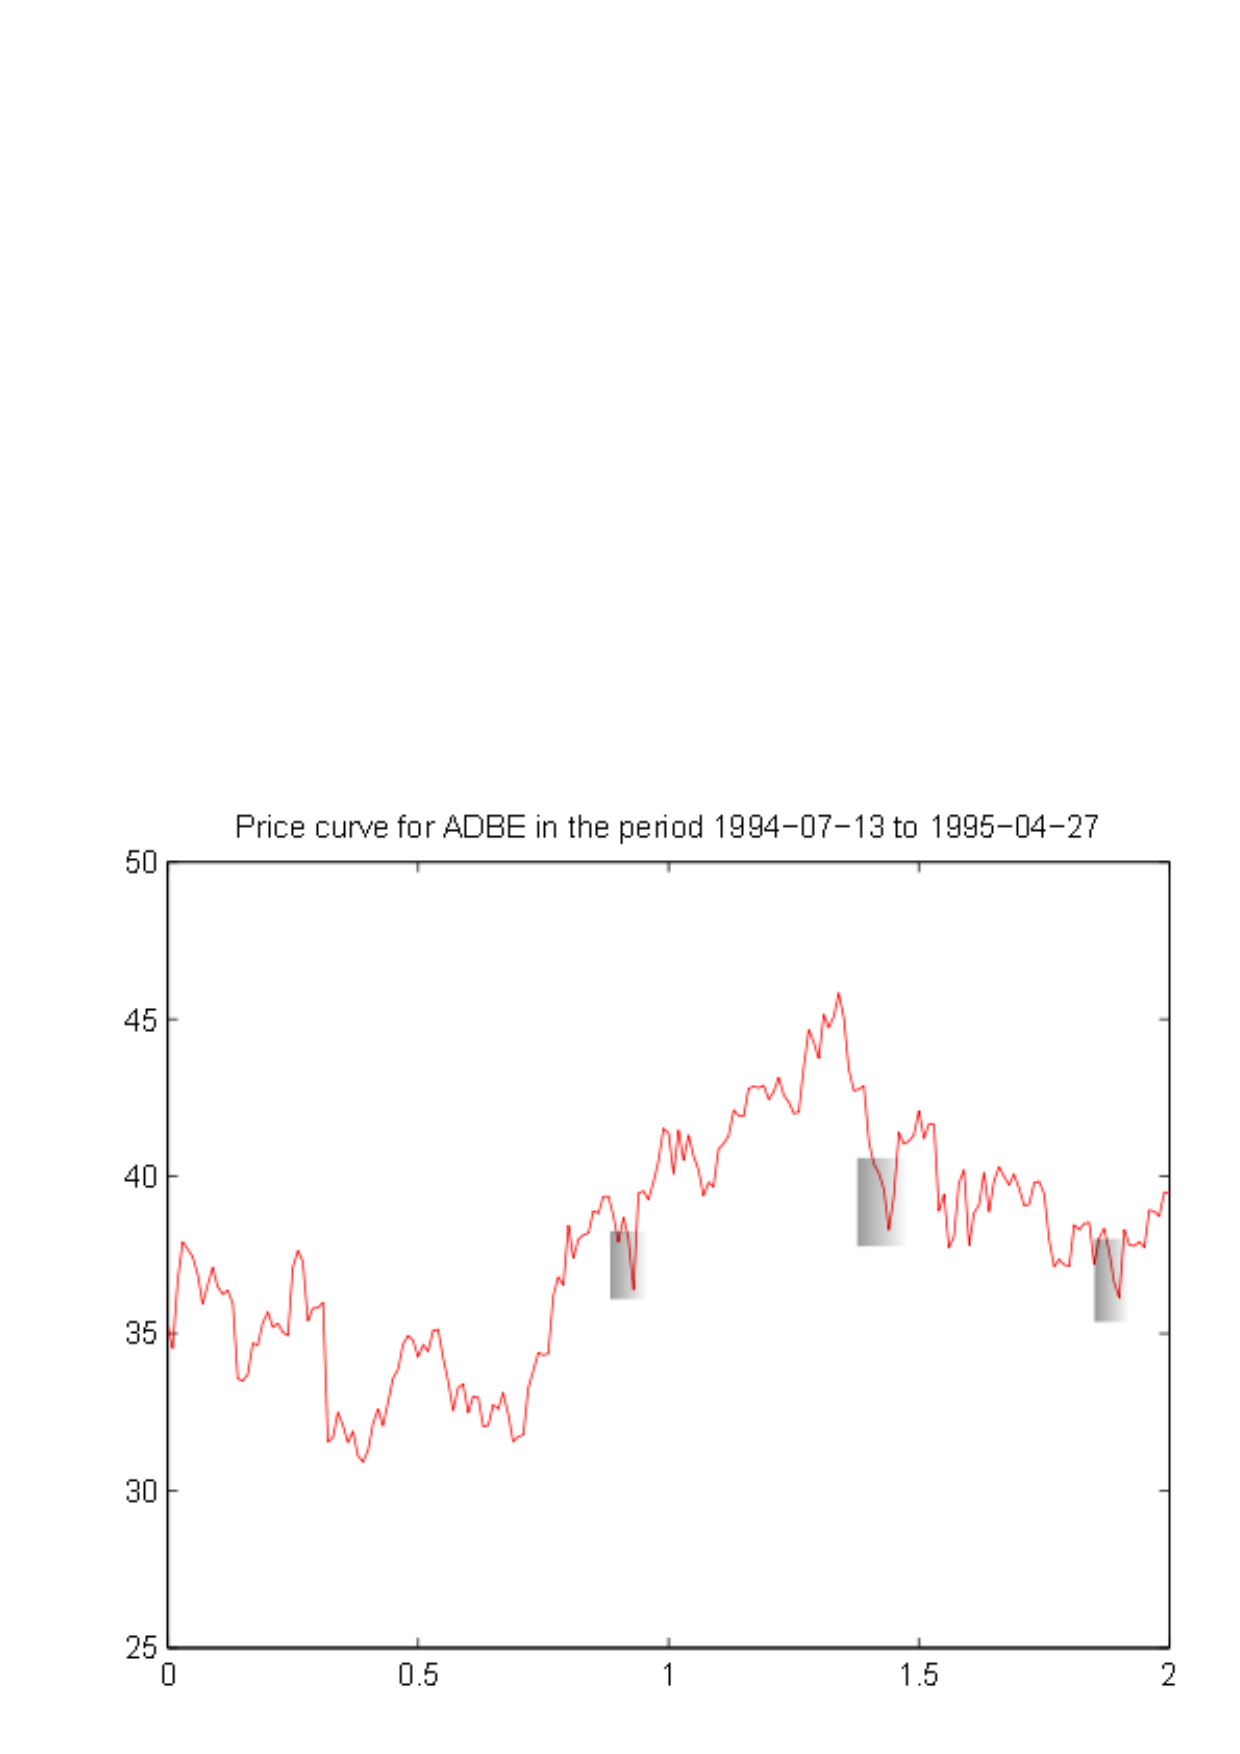
\includegraphics[scale=0.3]{ADBE_new.pdf}
\caption{Price movement for Adobe from 1994-07-13 to 1995-04-27.}
\label{fig:adbe}
\end{figure}

\subsection{General setting}
We consider the price movement of a given stock over a certain time period. We
divide the period in small subintervals of at least one day which we consider
data points in a sequence.  We label the data points such that the label
indicates the stock price movement. We use three distinct labels $F, H$ and $R$
indicating whether a given price will decrease its value over a given period
($F$), will retain approximately the same value ($H$), or will increase its
price ($R$). They are obtained depending on the opening and closing price for
the period. 
\subsection{A modified Apriori approach}
Formally, we are given a sequence $\mathbb{S}$ of symbols $s \in \mathcal{A}$ over some
alphabet $\mathbb{A}$. Let the support of a subsequence $S \subseteq
\mathbb{S}$ be $\mbox{sup}(S) = \frac{\#S}{|\mathbb{S}| - |S|}$ where $\#S$ is
the number of occurrences of the subsequence $S$ in $\mathbb{S}$ and
$|\mathbb{S}|$ and $|S|$ are the lengths of $\mathbb{S}$ and $S$, respectively.
That is, the support of a given sequence $S$ is the number of its occurrences
divided by the number of all subsequences in $\mathbb{S}$ of length $|S|$.  For
a given support threshold $\sigma$ and a confidence threshold $\tau$ we want to
find all subsequences $S \subset \mathbb{S}$ such that $\mbox{sup}(S) \geq
\sigma$ and $\mbox{conf}(S) \geq \tau$. The confidence $\mbox{conf}(S)$ of a
rule derived from $S$ is defined as
$\frac{\mbox{sup}(S)}{\mbox{sup}(S\backslash\ell)}$ where $\ell$ is the last
symbol in $S$.

The above definitions are similar to the itemset and transaction
setting in the classic frequent pattern mining context. However, an important
difference is that one can build only linearly many subsequences of a given
sequence, thus the following algorithm avoids the combinatorial explosion
caused by Apriori for lower support thresholds and is thus much more
efficient~\cite{fpstock}. 
\begin{algx} {Frequent sequence mining}
    \vspace{-5pt}
\begin{enumerate}
\setlength{\itemsep}{1pt}
\setlength{\parskip}{0pt}
\setlength{\parsep}{0pt}
\item Find frequent symbols, set $k=2$.
\item Join frequent subsequences of length $k-1$ if the last $k-2$ symbols of the first subsequence are identical to the first $k-2$ symbols of the second subsequence
\item build a set of candidates of length $k$ and filter out infrequent subsequences.
\item repeat steps 2--3 until no new frequent subsequences can be obtained.
\end{enumerate}
\end{algx}
\vspace{-6pt}
\begin{lemmx}
The algorithm correctly identifies all frequent subsequences of a given sequence.
\end{lemmx}
\textbf{Proof.} For a subsequence $S$ to be frequent the Apriori property that
all proper subsequences $S'$ of $S$ are frequent must hold. Thus, assuming we
have identified all frequent subsequences of length $k-1$, steps 2 and 3 return
a superset of the frequent subsequences of length $k$. Correctness follows by a
simple inductive argument. $\square$

{\bf Example:}  Let us consider a simple concrete example: the sequence $\mathcal{S} = abcbca ababca abccba abbabc bcacba$ contains 30 symbols. We are interested in all $k$-subsequences with frequency at least 0.15, i.e. occurring in at least 10\% of all subsequences of length $k$. The 1-subsequences are the symbols themselves and we find that all of them are frequent since they appear more than 4.5 times ($4.5 = 0.15\cdot 30$). Then we build candidate subsequences as $aa, ab, ac, ba, bb, bc, ca, cb, cc$ since they all satisfy the joining condition: the last 0 symbols of the first subsequence agree with the first 0 symbols of the second one. From these symbols we find that the subsequence $aa$ appears only once, $ab$ -- five times, $ac$ -- one time, $ba$ -- 4 times, $bb$ -- one time, $bc$-- 6 times, $ca$ -- three times, $cb$-- three times and $cc$ -- one time. The total number of 2-subsequences is 29, thus threshold is now $0.15 \cdot 29 = 4.35$. Thus, the frequent 2-subsequences are $ab$, $ba$ and $bc$. From these we build the following candidate 3-subsequences: $aba$, from $ab$ and $ba$, $bab$, from $ba$ and $ab$, and $abc$, from $ab$ and $bc$. Note that $ba$ and $bc$ can not be combined since they don't satisfy the joining condition. Now $aba$ appears only once, $bab$ twice, and $abc$ -- four times. Thus, no 3-subsequence is frequent, i.e. occur more than $4.2 = 0.15\cdot 28$ times, and the algorithm terminates.

In the very same way as in Apriori one computes the confidence of each rule.

\subsection{Results}
\subsubsection{Labeling}
We experimented with several values for the number of labels. It turns out that the more labels we have the more difficult it becomes to detect any frequent subsequences for a reasonable support threshold. Thus, we choose to present results when only three labels are used.  

As already mentioned, the three different labels $F, H$ and $R$ indicate whether the price will fall, remain relatively the same, or raise in the considered time period $t$, respectively. The labels are obtained in a natural way: given some threshold $\tau$, we compute the value $f:=\frac{c-o}{c}$ where $c$ is the closing price for the considered period $t$, and $o$ is the opening price. Note that we divide by $c$ in order to achieve normalization not depending on the absolute values of the stock price. Then we label $t$ as $H$ if $-\tau \leq f \leq \tau$, as $F$ if $f < -\tau$, and as $R$ otherwise. 

It is in general a difficult problem to choose an optimal threshold $\tau$, since choosing a small value will lead to labeling periods as either $F$ or $R$ even for non-significant changes of the stock price. On the other hand, big values of $\tau$ result in too many periods labeled as $H$ and this makes it difficult to mine rules with consequent different from $H$.  We observed that values of about $0.1$ give a balanced distribution among labels for most stocks for short time periods and allow the mining of reasonable amount of rules. 

We also experimented with labeling different time periods: it seems that for longer periods valuable information for price movements within the period is lost, while for some stocks for short periods like one day it is difficult to capture the effect of, say, more slowly price movement.  

\subsubsection{Choosing the best rule}
In certain situations we might be able to apply more than one rule. For example, the labels for the last three time periods are $HHF$ and we have the rules $HF \rightarrow F$ and $HHF \rightarrow H$. The most natural choice is the rule with the best confidence. However, a rule with a longer antecedent might give us better information since it takes into account more information. We implemented both strategies. It is difficult to say which one performs better, since apparently different stocks behave differently.  

\subsubsection{Average correctness}

After labeling the data for a given stock over a certain time period, say 3 days, we perform frequent sequence mining over the sequence. We use the first $2/3$ of the sequence for frequent pattern mining, and the last $1/3$ for applying our rules and correctness testing of our predictions. For all considered stocks we mined the sequences for the whole price history. 

The following table shows the label distribution and the percentage of correct predictions we obtain for certain stocks from the technology sector for threshold $\tau = 0.012$ and label period $t=2$. A more comprehensive list can be found in the appendix.
\begin{center}
\begin{tabular}{| l | l | l | l | l |}
\hline
Stock & average F & average R & average H & correct predictions\\
\hline
  AAPL & 0.3490 & 0.2935 & 0.3574 & 0.3888\\
\hline
  ADBE & 0.3476 & 0.2828 & 0.3695 & 0.3805 \\
\hline 
DELL & 0.32164 & 0.3154 & 0.3628 & 0.3823\\
\hline
  HPQ & 0.2973 & 0.3819 & 0.3207 & 0.3333 \\
\hline
MSFT & 0.2839 & 0.4013 & 0.3146 & 0.5702\\
\hline
WFR & 0.3988 & 0.2172 & 0.3839 & 0.4628\\
\hline
\end{tabular}
\end{center}

A similar table for the basic materials sector with $\tau = 0.009$ and $t=2$:
\begin{center}
\begin{tabular}{| l | l | l | l | l |}
\hline
Stock & average F & average R & average H & \% correct predictions\\
\hline
ADM & 0.38 & 0.248 & 0.3716 & 0.4006\\
\hline
AVP & 0.3516 & 0.2838 & 0.3644 & 0.3841\\
\hline
MKC & 0.2774 & 0.4095 & 0.3129 & 0.3435\\
\hline
NWL & 0.3618 & 0.2701 & 0.3680 & 0.4640\\
\hline
RAI & 0.2638 & 0.4146 & 0.3214 & 0.3846\\
\hline
TAP & 0.3192 & 0.3412 & 0.3394 & 0.3946\\
\hline
\end{tabular}
\end{center}

Different stocks behave differently and for example Microsoft turns out to be
much more predictive than Hewlett-Packard. Nevertheless, for all stocks the
percentage of correct predictions is significantly better than guessing at
random based solely on the labels distribution.  We observe that the higher
threshold $\tau$ we choose, i.e. we are more conservative in labeling a price
movement as $F$ or $R$, the better predictions we get. See Figure 2. This has
two explanations: First, most rules should have consequent $H$, thus simply
predicting $H$ for each next day should also give a good estimate. On the other
hand, as one clearly sees from the graphic the percentage of correct
predictions is growing faster than the percentage of $H$ labels. The intuitive
explanation is that the price movement becomes less sensitive to small
oscillations.
%We obtain the following results for chosen stocks:
\begin{figure}[htb!]
\caption{Correctness}
\centering%
\includegraphics[scale=0.7]{corr.pdf}
\end{figure}
\subsection{Can we become rich?}
One obvious question that arises is how to use the discovered knowledge to make
some profit. First of all, we would like to distinguish between {\em knowledge
discovery} and {\em use of the discovered knowledge}. An experienced investor
can use the mined rules in a much cleverer way and the primary goal of this
project is applying data mining techniques for discovering knowledge, not a
real world application of the discovered knowledge. Nevertheless, out of
curiosity, we implemented the following simple strategy: If our rule for the
next day predicts $R$ we buy 10 stocks in the morning and sell them in the
evening, thus our revenue is $10\cdot (close\_price - open\_price)$. Note that
since we are buying and selling stocks in the same day, the effect inflation
has on the stock price movement is minimized.  The revenues we obtained for
different stocks are shown below.

    \begin{center}
\begin{tabular}{| l | l | l || l | l | l |}
\hline
Stock & Prediction & Revenue & Stock & Prediction & Revenue\\
\hline
AAPL & 0.3765 & 207.3 & ADI & 0.3624 & 23.6\\
\hline
ADSK & 0.2866 & 13.6 &  ALTR & 0.3921 & 0\\
\hline
AMD & 0.3702 & -39.6 & BMC & 0.5142 & 55.19\\
\hline
DELL & 0.4773 & 0.0 & EMC & 0.3916 & -8.1\\
\hline
FFIV & 0.3609 & 157.2 & FLSR & 0.29 & -306.1\\
\hline
NVDA & 0.3315 & 33.5 & MSFT & 0.6155 & 0.0\\
\hline
\end{tabular}
    \end{center}

We wanted to check whether a more conservative labeling strategy would yield
better revenue. The Figure 3 table summarizes the average revenue over all 42
stocks in the technology sector. Despite some fluctuations, the average revenue
drops for higher values of $\tau$, i.e. more labels $H$.
% \begin{figure}[h!]
% \centering%
% \includegraphics[scale=0.7]{revenue.pdf}
% \vspace{-1cm}
% \caption{Average revenue depending on labeling strategy.}
% \end{figure}
% 
\section{Conclusions}
\label{sec:conclusion}

We have shown two methods for guiding the average investor using data mining.
Using supervised learning, we saw that using a simple buy \& hold strategy
outperformed a machine learning approach, indicating that average investors
should take a simple approach to investing and not try to overanalyze the
situation with technicals.

Our frequent pattern mining clearly shows that certain rules can be mined and
for most of the stocks they turn out to be to some degree accurate. However,
much deeper research is required in order to analyze which requirements should
a stock satisfy in order to obtain a reliable labeling. Apparently, simply
dividing stocks into sectors is not enough and more subtle subdivision needs to
be performed. It is in general questionable whether approaches based on
``purely" frequent pattern mining techniques can be successful since they only
take into account the price movement. A more promising direction would be to
use frequent pattern mining in combination with other techniques in order to
support the prediction based on other methods. But such a study is beyond the
scope of a course project.  
%\subsection{Correlation pattern mining}
%It is often the case that the price movement of a certain stock is correlated with the prices of other stocks. For example higher prices for metals will affect negatively the automotive industry but the effect occurs after some time. Another example is...
%
%Inspired by the above we implemented a sequence mining algorithm for detecting correlations between stocks within a given time span. For example is there a correlation between the price movement of stock $A$ in the interval $[p, q]$ and the price of stock $B$ in day $q+t$ for some appropriately chosen $t$. We experimented with different time intervals in order to mine dependencies between the stocks.

\begin{thebibliography}{1}
\small

\vspace{-0.25cm}
\bibitem{brock1992}
W.~Brock, J.~Lakonishok, and B.~LeBaron.
\newblock Simple technical trading rules and the stochastic properties of stock
  returns.
\newblock {\em The Journal of Finance}, 47(5):1731--1764, 1992.
\vspace{-0.25cm}

\bibitem{Weka}
Mark Hall, Eibe Frank, Geoffrey Holmes, Bernhard Pfahringer, Peter Reutemann,
Ian H. Witten. \newblock The WEKA Data Mining Software: An Update. \newblock
2009. SIGKDD Explorations, Volume 11, Issue 1. 
\vspace{-0.25cm}

\bibitem{fpstock}
Jo Ting, Tak-Chung Fu, Fu-Lai Chung: 
\newblock Mining of Stock Data: Intra- and Inter-Stock Pattern Associative Classification. \newblock {\em DMIN 2006:} 30--36
\vspace{-0.25cm}

\bibitem{vapnik2006estimation}
V.~Vapnik.
\newblock {\em Estimation of dependences based on empirical data}.
\newblock Springer-Verlag New York Inc, 2006.
\vspace{-0.25cm}

\bibitem{Yahoo}
Yahoo Finance.
\newblock \url{http://finance.yahoo.com}. 2011.

\end{thebibliography}

% 
% \section{Appendix}
% \begin{verbatim}
% AAPL.txt
% F : 0.29525483304042177
% H : 0.36379613356766255
% R : 0.3409490333919156
% correctness = 0.3888888888888889
% +++++++++++++++++++++++++++++++++++++++
% ADBE.txt
% F : 0.2827324478178368
% H : 0.40037950664136623
% R : 0.31688804554079697
% correctness = 0.3333333333333333
% +++++++++++++++++++++++++++++++++++++++
% ADI.txt
% F : 0.2972027972027972
% H : 0.4195804195804196
% R : 0.28321678321678323
% correctness = 0.271356783919598
% +++++++++++++++++++++++++++++++++++++++
% ADSK.txt
% F : 0.29891304347826086
% H : 0.3351449275362319
% R : 0.36594202898550726
% correctness = 0.36220472440944884
% +++++++++++++++++++++++++++++++++++++++
% ALTR.txt
% F : 0.31237322515212984
% H : 0.36511156186612576
% R : 0.3225152129817444
% correctness = 0.33557046979865773
% +++++++++++++++++++++++++++++++++++++++
% AMAT.txt
% F : 0.3087719298245614
% H : 0.3508771929824561
% R : 0.34035087719298246
% correctness = 0.368
% +++++++++++++++++++++++++++++++++++++++
% AMD.txt
% F : 0.4276206322795341
% H : 0.21963394342762063
% R : 0.3527454242928453
% correctness = 0.3786764705882353
% +++++++++++++++++++++++++++++++++++++++
% BMC.txt
% F : 0.2511111111111111
% H : 0.4288888888888889
% R : 0.32
% correctness = 0.5342465753424658
% +++++++++++++++++++++++++++++++++++++++
% BRCM.txt
% F : 0.3140794223826715
% H : 0.34296028880866425
% R : 0.34296028880866425
% correctness = 0.3333333333333333
% +++++++++++++++++++++++++++++++++++++++
% CPWR.txt
% F : 0.2557544757033248
% H : 0.4040920716112532
% R : 0.340153452685422
% correctness = 0.29285714285714287
% +++++++++++++++++++++++++++++++++++++++
% CTSH.txt
% F : 0.2564102564102564
% H : 0.38095238095238093
% R : 0.3626373626373626
% correctness = 0.41333333333333333
% +++++++++++++++++++++++++++++++++++++++
% CTXS.txt
% F : 0.2782874617737003
% H : 0.3302752293577982
% R : 0.39143730886850153
% correctness = 0.2916666666666667
% +++++++++++++++++++++++++++++++++++++++
% DELL.txt
% F : 0.3216494845360825
% H : 0.3154639175257732
% R : 0.3628865979381443
% correctness = 0.38235294117647056
% +++++++++++++++++++++++++++++++++++++++
% EMC.txt
% F : 0.3054393305439331
% H : 0.3410041841004184
% R : 0.35355648535564854
% correctness = 0.34210526315789475
% +++++++++++++++++++++++++++++++++++++++
% ERTS.txt
% F : 0.33555555555555555
% H : 0.35333333333333333
% R : 0.3111111111111111
% correctness = 0.3805309734513274
% +++++++++++++++++++++++++++++++++++++++
% FFIV.txt
% F : 0.2896825396825397
% H : 0.28174603174603174
% R : 0.42857142857142855
% correctness = 0.2777777777777778
% +++++++++++++++++++++++++++++++++++++++
% FSLR.txt
% F : 0.3010752688172043
% H : 0.3978494623655914
% R : 0.3010752688172043
% correctness = 0.2982456140350877
% +++++++++++++++++++++++++++++++++++++++
% HPQ.txt
% F : 0.24383301707779886
% H : 0.43833017077798864
% R : 0.3178368121442125
% correctness = 0.3333333333333333
% +++++++++++++++++++++++++++++++++++++++
% INTC.txt
% F : 0.27547169811320754
% H : 0.44528301886792454
% R : 0.2792452830188679
% correctness = 0.2962962962962963
% +++++++++++++++++++++++++++++++++++++++
% INTU.txt
% F : 0.21558441558441557
% H : 0.44935064935064933
% R : 0.33506493506493507
% correctness = 0.3014705882352941
% +++++++++++++++++++++++++++++++++++++++
% KLAC.txt
% F : 0.3422222222222222
% H : 0.31333333333333335
% R : 0.34444444444444444
% correctness = 0.2641509433962264
% +++++++++++++++++++++++++++++++++++++++
% LLTC.txt
% F : 0.29777777777777775
% H : 0.3977777777777778
% R : 0.30444444444444446
% correctness = 0.3488372093023256
% +++++++++++++++++++++++++++++++++++++++
% LSI.txt
% F : 0.3634361233480176
% H : 0.2687224669603524
% R : 0.36784140969163
% correctness = 0.36
% +++++++++++++++++++++++++++++++++++++++
% MHCP.txt
% F : 0.2927461139896373
% H : 0.40932642487046633
% R : 0.2979274611398964
% correctness = 1.0
% +++++++++++++++++++++++++++++++++++++++
% MSFT.txt
% F : 0.2718808193668529
% H : 0.4692737430167598
% R : 0.25884543761638734
% correctness = 0.5702479338842975
% +++++++++++++++++++++++++++++++++++++++
% MU.txt
% F : 0.4157782515991471
% H : 0.2260127931769723
% R : 0.3582089552238806
% correctness = 0.38181818181818183
% +++++++++++++++++++++++++++++++++++++++
% NOVL.txt
% F : 0.29545454545454547
% H : 0.4256198347107438
% R : 0.27892561983471076
% correctness = 0.3305785123966942
% +++++++++++++++++++++++++++++++++++++++
% NSM.txt
% F : 0.34609250398724084
% H : 0.34290271132376393
% R : 0.31100478468899523
% correctness = 0.3473053892215569
% +++++++++++++++++++++++++++++++++++++++
% NTAP.txt
% F : 0.2978723404255319
% H : 0.2765957446808511
% R : 0.425531914893617
% correctness = 0.3644067796610169
% +++++++++++++++++++++++++++++++++++++++
% NVDA.txt
% F : 0.32950191570881227
% H : 0.2796934865900383
% R : 0.39080459770114945
% correctness = 0.33884297520661155
% +++++++++++++++++++++++++++++++++++++++
% NVLS.txt
% F : 0.35777777777777775
% H : 0.27555555555555555
% R : 0.36666666666666664
% correctness = 0.4090909090909091
% +++++++++++++++++++++++++++++++++++++++
% ORCL.txt
% F : 0.27111111111111114
% H : 0.4177777777777778
% R : 0.3111111111111111
% correctness = 0.460431654676259
% +++++++++++++++++++++++++++++++++++++++
% RHT.txt
% F : 0.27309236947791166
% H : 0.3855421686746988
% R : 0.3413654618473896
% correctness = 0.2682926829268293
% +++++++++++++++++++++++++++++++++++++++
% SAI.txt
% F : 0.16842105263157894
% H : 0.6736842105263158
% R : 0.15789473684210525
% correctness = 0.6666666666666666
% +++++++++++++++++++++++++++++++++++++++
% SNDK.txt
% F : 0.3556231003039514
% H : 0.22188449848024316
% R : 0.42249240121580545
% correctness = 0.3935483870967742
% +++++++++++++++++++++++++++++++++++++++
% SYMC.txt
% F : 0.3
% H : 0.4177777777777778
% R : 0.2822222222222222
% correctness = 0.2894736842105263
% +++++++++++++++++++++++++++++++++++++++
% TER.txt
% F : 0.3688888888888889
% H : 0.26222222222222225
% R : 0.3688888888888889
% correctness = 0.3680555555555556
% +++++++++++++++++++++++++++++++++++++++
% TXN.txt
% F : 0.3
% H : 0.37555555555555553
% R : 0.3244444444444444
% correctness = 0.24675324675324675
% +++++++++++++++++++++++++++++++++++++++
% VRSN.txt
% F : 0.23843416370106763
% H : 0.4199288256227758
% R : 0.3416370106761566
% correctness = 0.273972602739726
% +++++++++++++++++++++++++++++++++++++++
% WDC.txt
% F : 0.36
% H : 0.24888888888888888
% R : 0.39111111111111113
% correctness = 0.46875
% +++++++++++++++++++++++++++++++++++++++
% WFR.txt
% F : 0.39880952380952384
% H : 0.21726190476190477
% R : 0.38392857142857145
% correctness = 0.4628099173553719
% +++++++++++++++++++++++++++++++++++++++
% XLNX.txt
% F : 0.28314606741573034
% H : 0.36404494382022473
% R : 0.35280898876404493
% correctness = 0.31958762886597936
% \end{verbatim}
% 
\end{document}
